\subsection{Implementation of Ruder style transfer for video}
\label{sec:Ruder style transfer}
As a part of our project we have implemented some of the components described in the paper by Ruder et al. \cite{Ruder:1}. Here we try to reduce the noise that appears when styling each image independently by introducing a temporal constraint in order to penalize the model for straying too far away from the previous image.\newline\newline
The temporal constraint we have implemented is an additional loss-component: \newline

\begin{equation}
\mathcal{L}_{temporal}(x, \omega, c) = \frac{1}{D}\sum_{k=1} c_k \cdot (x_k - \omega_k)^2
\end{equation}
Since we are using the style and content-loss used in Gatys style transfer, our total loss-function with a shortterm temporal constraint is this:\newline
\begin{equation}
\mathcal{L}_{shortterm}(p^{(i)}, a, x) = \alpha \mathcal{L}_{content} + \beta \mathcal{L}_{style} + \gamma \mathcal{L}_{temporal}(x^{(i)}, \omega_{i-1}^i(x^{i-1}, c^{i-1, i}))
\end{equation}
We use different weights for different resolutions, generally increasing the style-loss and decreasing the temporal constraint with increasing resolution.\newline
As well as using this shortterm temporal loss function, we also initialize every frame after the first stylized frame with the previously stylized frame \textit{i-1} warped to the current image \texit{i}. This is done by using the flow between the content image $i-1$ and $i$. 
To calculate this flow we need a flow algorithm. In our implementation we have used cv2's DeepFlow function. The calculated flow between frames is also used to create our c-matrix using the inequalities described in Section \ref{sec:usage_of_optical_flow}. These inequalities result in c-matrix masks like these:\newline 
\begin{figure}[!ht]
\begin{center}
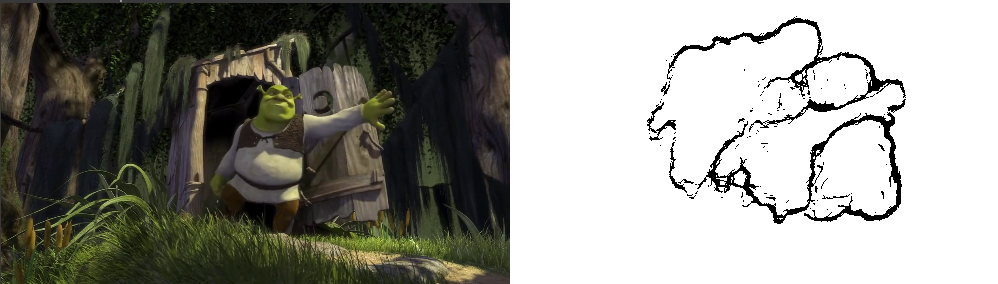
\includegraphics[scale=0.35]{report/Method/images/shrek_flow.png}
\caption{A frame from the shrek video and the flow image calculated, indicating what parts of the image are moving and should be recalculated}
\label{fig:architecture}
\end{center}
\end{figure}
\newline
To calculate these values for each frame, we have primarily used the numpy library. We have also implemented the long-term temporal constraint described in Section \ref{sec:long_term_temporal_loss}. However, a lot of additional computation is needed for this. With our current access to hardware and the negligible results we got from testing our implementation, we decided to not use this in our results.\newline\newline
With the implemented temporal constraint, we are able to have some consistency between frames, resulting in less noise: \newline
\begin{figure}[!ht]
\begin{center}
\includegraphics[scale=0.11]{report/Method/images/ruder.png}
\caption{Two consecutive frames produced by Ruders method using La Muse (Picasso) as style refernce, source video is from Parasite}
\label{fig:architecture}
\end{center}
\end{figure}In figure \ref{fig:architecture} we can see the same artifacts staying in the same place in both adjacent frames, while the person to the left has moved. The results from this implementation can be seen in \ref{seq:ruder_result}